\documentclass[12pt,reqno]{article}
\usepackage[dutch]{babel}
\usepackage[margin=1.2in]{geometry}
\usepackage{amsmath}
\usepackage{amssymb}
\usepackage{color}
\usepackage{tikz}
\usepackage{url}

\title{\textbf{Congruente getallen}\\
		\small{eerste versie studentencheck}}
\author{
	\begin{tabular}{ l l }
		Lotte Bruijnen, & 4297652 \\
		Daan van Laar, & 5518741 \\
		Suzanne Vincken, & 4273338
	\end{tabular}\\
	Onder begeleiding van: Carel Faber, UU
}
\date{10-12-2015}

\newcommand*{\NN}{\ensuremath{\mathbb{N}}}
\newcommand*{\ZZ}{\ensuremath{\mathbb{Z}}}
\newcommand*{\QQ}{\ensuremath{\mathbb{Q}}}
\newcommand*{\RR}{\ensuremath{\mathbb{R}}}
\newcommand*{\CC}{\ensuremath{\mathbb{C}}}
\newcommand*{\QED}{\hfill\ensuremath{\blacksquare}}

\begin{document}
	\maketitle
	\allowdisplaybreaks
	
	
	\section{Inleiding}
	We gaan het hebben over congruente getallen. Eerst vindt u een begrippenlijst, zodat u de betekenis van veelvoorkomende begrippen altijd op kan zoeken. Daarna wordt er uitgelegd wat congruente getallen zijn en wat dit te maken heeft met Pythagore\"ise drietallen. We gaan kijken hoe we alle congruente getallen kunnen vinden en daarna zullen we ook kijken naar een aantal belangrijke stellingen/bewijzen.
	
	\textit{Als er tekst roodgekleurd is, moeten we het bewijs nog afmaken, of nagaan of de uitspraak waar is.}
	
	
	\section{Begrippen}
	\begin{tabular}{ p{4,6cm} p{10cm} }
		\textbf{Kwadraatvrij}: \cite{Beukers} & Een kwadraatvrij getal is een getal dat niet deelbaar is door een kwadraat groter dan $1$. Waarbij een kwadraat een getal $k\in\NN$ zodat $\sqrt{k}\in\NN$. \\
		\textbf{Primitieve congruente getallen}: & Een kwadraatvrij congruent getal. \\
		%\textbf{begrip}: & uitleg \\
		%\textbf{begrip}: & uitleg
	\end{tabular}
	
	
	\newpage
	\section{Congruente getallen en Pythagore\"{i}se drietallen}	
	Eerst zullen we kijken naar de definitie van congruente getallen. Er bestaan echter meerdere definities. We zullen er hier twee behandelen.\\
	
	Ten eerste kijken we naar de meetkundige definitie uit \cite{Oort}[p.3]:	
	\newtheorem{CGm}{Defenitie}
	\begin{CGm}
		Een positief geheel getal $n$ heet een congruent getal als er een rechthoekige driehoek bestaat met lengtes van zijden in $\QQ_{>0}$ en met oppervlak gelijk aan $n\in\ZZ$. Noem de lengtes van de zijden $x,y,z\in\QQ$; met behulp van de stelling van Pythagoras zien we:
		\begin{figure*}[h!]
			\centering
			\begin{tikzpicture}[xscale=6, yscale=3]
			\coordinate (O) at (0,0);
			\coordinate (A) at (1,0);
			\coordinate (B) at (0,1);
			\draw (O) -- node[auto,swap]{$x$} 
			(A) -- node[auto,swap]{$z$}
			(B) -- node[auto,swap]{$y$} (O);
			\coordinate (M) at (1.5, 0.5);
			\draw (M) node[auto]{$x\cdot y/2 = n$};
			\coordinate (N) at (1.5, 0.25);
			\draw (N) node[auto]{$x^2 + y^2 = z^2$};
			\end{tikzpicture}
		\end{figure*}
	\end{CGm}
	We zien dat hier een congruent getal $n$ wordt gegeven als de oppervlakte van een rechthoekige driehoek met zijn in $\QQ$. We kunnen conguente getallen ook bekijken via een algebra\"{i}sche benadering. De volgende definitie komt van \cite{Oort}[p.3].
	
	\newtheorem{CGa}{Defenitie}
	\begin{CGa}
		Een positief geheel getal $n$ heet een congruent getal als er bestaat een $\delta\in\QQ$ zodanig dat
		\begin{align*}
		\delta^2 - n, \delta^2, \delta^2 + n
		\end{align*}
		kwadraten zijn in $\QQ$.
	\end{CGa}	
	Een getal dat aan deze definitie voldoet is het getal 5. We nemen $\delta = \frac{41}{12}$. Dan geldt:
	\begin{align*}
	\delta^2 &= \left( \frac{41}{12} \right)^2 \in\QQ\\
	\delta^2 - n &= \frac{1681}{144} - 5 = \frac{961}{144} = \left( \frac{31}{12}\right)^2 \in\QQ\\
	\delta^2 + n &= \frac{1681}{144} + 5 = \frac{2401}{144} = \left( \frac{48}{12}\right)^2 \in\QQ
	\end{align*}
	Hieruit volgt dus dat $5$ een conguent getal is. \\
	
	%Een andere manier om congruente getallen te defini\"{e}ren is door er op een meetkundige manier naar te kijken. Echter, voor die definitie is het handig om eerst te kijken naar Pythagore\"ische drietallen. \\
	
	%Dit straks verwijderen en de definities weer omdraaien.
	Bij de eerste definitie maken we gebruik van Pythagore\"ische drietallen. Daar zullen we nu wat meer over uitleggen.\\
	
	De geschiedenis van Pythagore\"ische drietallen begint bij het vermoeden van Fermat. Dit vermoeden ziet er als volgt uit:
	\begin{align}
	x^n + y^n = z^n \qquad \text{met} \qquad n \in \NN.
	\end{align}
	Fermat vermoedde dat voor $n \geq 3$ er alleen triviale oplossingen bestaan voor (1). Dat wil zeggen, $\forall (x,y,z) \in \ZZ^3$ en $x^n + y^n = z^n$ met $n \geq 3$, geldt $x \cdot y \cdot z = 0$. \\
	Wij zijn echter vooral ge\"interesseerd in het geval waarbij $n=2$ en alle niet triviale oplossingen van de vergelijking $x^2 + y^2 = z^2$. Deze oplossingen noteren we als $(x,y,z)$ en we noemen deze oplossingen Pythagore\"ische drietallen. Dit komt omdat het vermoeden van Fermat met $n=2$ de stelling van Pythagoras is. De niet-triviale oplossingen $(x,y,z)$ van $x^2 + y^2 = z^2$ vormen dan ook een rechthoekige driehoek waarbij $z$ de schuine zijde is. Een simpel voorbeeld van een Pythagore\"{i}sch drietal is $(3,4,5)$, want $3^2 + 4^2 = 9 + 16 = 25 = 5^2$. \\
	Een speciaal soort Pythagore\"isch drietal is het zogenaamde primitieve Pythagore\"ische drietal. Dit is een Pythagore\"isch drietal $(x,y,z)$ waarvoor ook geldt dat $ggd(x,y)=1$.
	{\color{red}Bewijs dat ggd(x,z) en ggd(y,z) ook 1 zijn. Nog veel meer bewijzen over ppd's.}
	%Tweede definitie congruente getallen
	
	
	\section{Voorbeelden}
	Hieronder volgen drie voorbeelden van congruente getallen, volgens definitie 1. Het kleinste congruente getal is $5$. Dat is de driehoek met de volgende zijden:
	\begin{figure*}[h!]
		\centering
		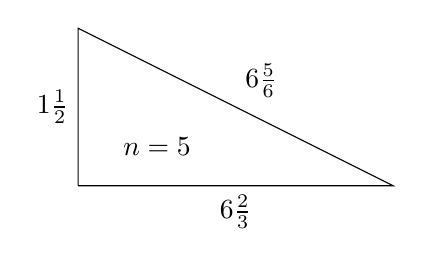
\begin{tikzpicture}[xscale=4, yscale=2]
		\coordinate (O) at (0,0);
		\coordinate (A) at (1,0);
		\coordinate (B) at (0,1);
		\coordinate (M) at (0.25, 0.25);
		\draw (O) -- node[auto,swap]{$6\frac{2}{3}$} 
		(A) -- node[auto,swap]{$6\frac{5}{6}$}
		(B) -- node[auto,swap]{$1\frac{1}{2}$} (O);
		\draw (M) node[auto]{$n=5$};
		\end{tikzpicture}
	\end{figure*}\\
	Het kleinste congruente getal met zijden uit $\NN$ is $6$. Dat is de driehoek met de volgende zijden:
	\begin{figure*}[h!]
		\centering
		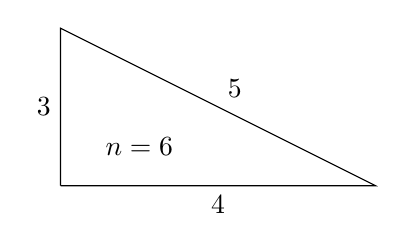
\begin{tikzpicture}[xscale=4, yscale=2]
		\coordinate (O) at (0,0);
		\coordinate (A) at (1,0);
		\coordinate (B) at (0,1);
		\coordinate (M) at (0.25, 0.25);
		\draw (O) -- node[auto,swap]{$4$} 
		(A) -- node[auto,swap]{$5$}
		(B) -- node[auto,swap]{$3$} (O);
		\draw (M) node[auto]{$n=6$};
		\end{tikzpicture}
	\end{figure*}\\
	Dit is de driehoek met oppervlakte $157$: \cite{Koblitz}[p.5]
	\begin{figure*}[h!]
		\centering
		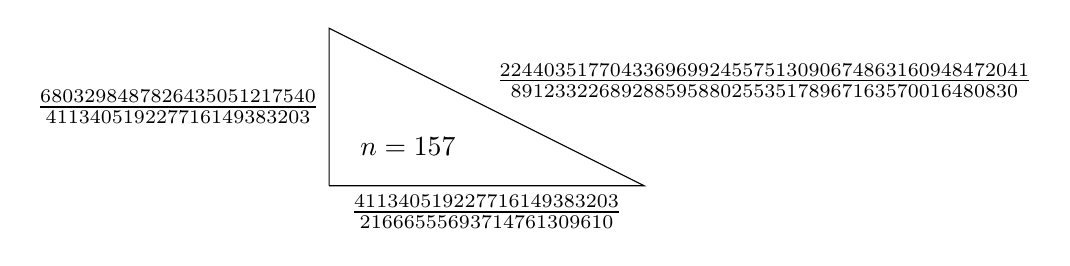
\begin{tikzpicture}[xscale=4, yscale=2]
		\coordinate (O) at (0,0);
		\coordinate (A) at (1,0);
		\coordinate (B) at (0,1);
		\coordinate (M) at (0.25, 0.25);
		\draw (O) -- node[auto,swap]{$\frac{411340519227716149383203}{21666555693714761309610}$} 
		(A) -- node[auto,swap]{$\frac{224403517704336969924557513090674863160948472041}{8912332268928859588025535178967163570016480830}$}
		(B) -- node[auto,swap]{$\frac{6803298487826435051217540}{411340519227716149383203}$} (O);
		\draw (M) node[auto]{$n=157$};
		\end{tikzpicture}
	\end{figure*}
	
	
	\section{Congruente getallen vinden}
	Het volgende komt uit \cite{Koblitz}[p.3-4].\\
	We weten nu dat een een congruent getal $n$ een geheel getal is als oppervlakte van een driehoek met rationale zijden. Als we nu willen kijken welke $n'\in\NN$ congruente getallen zijn, moeten we heel $\NN$ door. Dit is niet te doen. Daarom willen we het aantal mogelijke waardes van $n'$ beperken. We doen het volgende:\\
	Neem een getal $r\in\QQ$ en zeg $r$ is congruent. Dan zijn $x,y,z\in\QQ$ de zijden van de rechthoekige driehoek met oppervlakte $r$. We kunnen nu voor elke $r\neq0$ een $s\in\QQ$ vinden zodat $s^2r$ een kwadraatvrij natuurlijk getal is.
	\begin{itemize}
		\item[] \underline{Bewijs}: We weten $r\in\QQ$, dus $r$ is te schrijven als: $r=\frac{p}{q}$. Neem nu een $s\in\QQ$ zodat $s^2$ deelbaar is door $q$. {\color{red}Nu geldt dat $s^2r$ een kwadraatvrij getal.}\QED
	\end{itemize}
	We weten nu dat $s^2r$ een kwaadraatvrij getal is. En we doen het volgende: neem de driehoek met zijden $sx,sy,sz$. De oppervlakte van deze driehoek is $s^2r$. We kunnen nu zonder verlies van algemeenheid zeggen dat $s^2r=n$. We kunnen dus ook aannemen dat $n$ een congruent kwadraatvrij natuurlijk getal, oftewel een primitief congruent getal, is. We weten dan ook dat $s^2n$, met $s^2\in\QQ$, een congruent getal is.  \\
	
	We hebben hierboven gezien dat we de mogelijke waardes van $n'$ hebben beperkt, omdat $n'$ nu een kwadraatvrij getal is. Dus we kunnen nu al een stuk sneller door $\NN$ om te kijken welke getallen $n'\in\NN$ congruent zijn. Sterker nog: er betstaat een algoritme die voor elke $n'$ checkt of er een Pythagorees drietal bestaat zodat $n'$ de oppervlakte is van deze driehoek (dus $n'=n$). Als $n'$ congruent is, zet het algoritme deze in een lijst. Het probleem hierbij is dat we niet weten hoe lang we moeten zoeken naar een Pythagorees drietal die bij $n'$ past. Dus als $n'$ niet in de lijst staat, weten we niet of (1) $n'$ geen congruent getal is of (2) dat het zoeken te lang duurde en het zoeken is afgebroken. Wat we dus eigenlijk willen, is een gesloten formule vinden, zodat we makkelijk kunnen checken of $n'$ een congruent getal is of niet.\\
	
	We kunnen met de theorie van Tunnnell precies controleren welke pythagore\"ise drietallen bij een congruent getal horen. Hiervoor moeten we wel iets aannemen wat te maken heeft met elliptische krommen. Gebruik makend van de elliptische krommen, moet gelden dat een paar rationele getallen $(x,y)$ van een congruente driehoek met zijden $x,y,z$, moet voldoen aan de vergelijking: $y^2=x^3-n^2x$.
	
	
	\section{Presentaties van congruente getallen}
	We weten al dat ieder congruent getal afhangt van een Pythagore\"isch drietal, welke de presentatie wordt genoemd. Maar is dat een uniek drietal? En zo niet, hoeveel presentaties zijn er dan? Dat zijn de vragen waar we nu naar gaan kijken.\\
	
	Belangrijk is dat we eerst op \'e\'en lijn zitten, aangaande wat wel een Pythagore\"isch drietal is. Hier is een Pythagore\"isch drietal van de vorm $(x,y,z)$, waarbij $x,y,z\in \QQ_{>0}$ en $x^2 + y^2 = z^2$. Het bijbehorende congruente getal noemen we $N$, waarbij uiteraard geldt dat $N\in \QQ_{>0}$ (immers, $N = xy / 2$).\\
	
	Het is dus ook niet moeilijk te zien dat een congruent getal meerdere presentaties kan hebben. Neem bijvoorbeeld het getal 210, een presentatie daarvan is $(20,21,29)$, immers $(20\cdot 21)/2 = 210$. Een andere presentatie is $(12,35,37)$. En hoewel dit slechts \'e\'en getal is, is het desalniettemin zeer aannemelijk dat ieder congruent getal meerdere presentaties heeft. Sterker nog, ieder congruent getal heeft oneindig veel presentaties.\\
	
	Met de huidige definitie van "presentatie" is dat moeilijk na te gaan. Om het allemaal wat makkelijker te maken, gebruiken we een nieuwe definitie, gebaseerd op {\color{red}de stelling van Euclides}. We kiezen het positieve gehele getal $D$ dan zo dat $N=m\cdot n \cdot (m-n)^2/D^2$ een primitief congruent getal is. Hierbij zijn $m$ en $n$ zoals in de stelling van Euclides. (Ter herinnering: $m>n$, $ggd(m,n) = 1$ en $m+n$ is oneven.) Daarnaast geldt dat $x = m^2 - n^2$, $y = 2mn$ en $z = m^2 + n^2$.) In dit geval is de presentatie van het congruente getal dan $((m,n),D,N)$. Immers $D^2N = m\cdot n \cdot (m-n)^2$ en $xy/2 = D^2N$.\\
	
	Om nu te bewijzen dat ieder congruent getal oneindig veel presentaties heeft, moeten we eerst wat rekenwerk doen. We defini\"eren eerst:
	\begin{equation}
		U:= z^2=(m^2+n^2)^2, \qquad V:= 2xy=2(m^2-n^2)2mn
	\end{equation}
	Dit zijn de bouwstenen waar we straks een nieuwe presentatie mee gaan vormen voor ons congruente getal. Dat doen we als volgt:
	\begin{align}
			U\cdot V \cdot (U-V) \cdot (U+V)=\\
			z^2\cdot 2xy\cdot (y^2+y^2-2xy)\cdot (x^2+y^2+2xy)=\\
			2xy\cdot z^2\cdot (x-y)^2\cdot (x+y)^2=\\
			\{2\cdot z\cdot D\cdot (x-y)\cdot (x+y)\}^2\cdot N
	\end{align}
	We hebben zo een nieuwe presentatie gevonden van $N$, waarbij een nieuw Pythagore\"isch drietal hoort (voor het gemak $(a,b,c)$ genoemd). Hierbij geldt:
	\begin{equation}
		U'=c^2, \qquad V'=2ab, \qquad E=|\{2\cdot z\cdot D\cdot (x-y)\cdot (x+y)\}|
	\end{equation}
	Wat opvalt is dat $E>D$.\\
	
	We kunnen deze methode herhalen met $U'$, $V'$ en $E$, en zo weer een nieuwe presentatie vinden. Met die nieuwe presentatie kunnen we weer een nieuwe presentatie vinden, enzovoort. In feite kunnen we het dus oneindig vaak herhalen, waarbij we steeds een nieuwe presentatie vinden. Ergo: ieder congruent getal bevat oneindig veel presentaties.
	
	
	\section{Stellingen}
	{\color{red}Deze stellingen moeten we nog invoegen.}
	\newtheorem{Tunnell}{Theorem}
	\begin{Tunnell}
		\cite{Koblitz}[p.212] (Tunnell, 1983) If $n$ is a squarefree and odd (respectively, even) positive integer ans $n$ is the area of a right triangle with rational sides, then
		\begin{align}
		\#\{x,y,z\in\ZZ|n=2x^2+y^2+32z^2\} = \frac{1}{2}\#\{x,y,z\in\ZZ|n=2x^2+y^2+8z^2\}\\
		\notag \text{(respectively, } \\
		\#\{x,y,z\in\ZZ|\frac{n}{2}=4x^2+y^2+32z^2\} = \frac{1}{2}\#\{x,y,z\in\ZZ|\frac{n}{2}=4x^2+y^2+8z^2\})
		\end{align}
		If the weak Birch-Swinnerton-Dyer conjecture is true for the elliptic curves $E_n:y^2=x^3-n^2x$, then, conversely, these equalities imply that $n$ is a congruent number.
	\end{Tunnell}
	
	\newtheorem{Prop1}{Propositie}
	\begin{Prop1}
		\cite{Koblitz}[p.4] Let $n$ be a fixed squarefree positive integer. Let $X,Y,Z,x$ always denote rational numbers, with $X<Y<Z$. There is a one-to-one correspondence between right triangles with legs $X$ and $Y$, hypotenuse $Z$, and area $n$; and numbers $x$ for which $x$, $x+n$, and $x-n$ are each the square of a rational number. The correspondence is:
		\begin{align*}
		X,Y,Z\rightarrow x &= (Z/2)^2 \\
		x\rightarrow X &= \sqrt{x+n} - \sqrt{x-n}, Y = \sqrt{x+n}+\sqrt{x-n}, Z = 2\sqrt{x}.
		\end{align*}
		In particular, $n$ is a congruent number if and only if there exists $x$ such that $x$, $x+n$, and $x-n$ are squares of rational numbers.
	\end{Prop1}
	
	
	\bibliographystyle{plain}
	\bibliography{bib}
\end{document}